\documentclass[a4paper]{article}

%% Language and font encodings
\usepackage[english]{babel}
\usepackage[utf8x]{inputenc}
\usepackage[T1]{fontenc}

%% Sets page size and margins
\usepackage[a4paper,top=3cm,bottom=2cm,left=3cm,right=3cm,marginparwidth=1.75cm]{geometry}

%% Useful packages
\usepackage{amsmath}
\usepackage{amsfonts}
\usepackage{amssymb}
\usepackage{graphicx}
\usepackage{subcaption}
\usepackage[colorinlistoftodos]{todonotes}
\usepackage[colorlinks=true, allcolors=blue]{hyperref}

\graphicspath{ {figures/} }

% Commands
\newcommand{\alphabet}{\mathcal{A}}
\newcommand{\fullAlignment}{\mathbf{Y}}
\newcommand{\alignmentColumn}{\mathbf{y}}
\newcommand{\alignmentColumnRV}{Y}
\newcommand{\siteSplit}{\tilde{s}}
\newcommand{\siteSplitSet}{\mathcal{S}}
\newcommand{\fullAncestralStates}{\mathbf{H}}
\newcommand{\ancestralStateColumn}{\mathbf{h}}
\newcommand{\ancestralStateColumnRV}{H}
\newcommand{\ancestralSplit}{\tilde{h}}
\newcommand{\ancestralSplitSet}{\mathcal{H}}
\newcommand{\ancestralSplitPartition}{\eta}
\newcommand{\fullAncestralSplitPartitions}{\boldsymbol\eta}

\newcommand{\patternToSplit}{\psi}
\newcommand{\ancestralToSplit}{\xi}

\newcommand{\siteSplitRV}{\Psi}
\newcommand{\ancestralSplitRV}{\Xi}

\newcommand{\nCols}{n}
\newcommand{\nSiteRows}{m}
\newcommand{\nAncestralStateRows}{p}
\newcommand{\nSiteSplits}{q}
\newcommand{\nAncestralSplits}{r}

\newcommand{\shannonDivergence}{D}

\allowdisplaybreaks

\title{Possible Inconsistency in Maximum Likelihood Calculation of Ancestral States}
\author{Shaw, Matsen, Minin}

\begin{document}
\maketitle

%comments from Erick:
% >  This is great!
% > - would be great to have all the calculations showing the "refinement" structure written out for the various tree structures (just done by hand and scanned is just fine)
% > - I think of the "refinement" as a partition, so perhaps rather than "empty refinement" we have a "single-element partition"
% > - in order to interpret the site patterns I need to figure out in what order the leaves are labeled
% > - how is ell calculated?
% > - on the numerical sanity check, it doesn't seem clear that the branch lengths can be different than the inferred ones-- they can!
% > - re "general case", agreed though I don't think that we need numerical optimization of branch lengths in a set of a branch length partition-- we can just get the optimal branch length directly. Namely, for each branch, we know all hidden states (given that we are in a set of a partition) and so can count the number of mutations across that branch. From there we have a simple likelihood function, which either has an optimal in the interior or on the boundary of the partition.

\renewcommand{\arraystretch}{1.2} % because otherwise exponents get eaten by \hline


\section*{Introduction}

Classical maximum-likelihood (ML) estimation in phylogenetics operates by integrating out possible ancestral states at the internal nodes of the tree.
Recently \cite{Neher2017} have suggested using an approximation to ML inference in which the likelihood is maximized jointly across model parameters and ancestral sequences.
This is attractive from a computational perspective: such joint ML inference can proceed according to an iterative procedure in which ML ancestral sequences are first inferred and then model parameters are optimized conditional on the ancestral sequences.
This latter step is simpler and more computationally efficient when conditioning on ancestral sequences compared to the case in which ancestral sequences are marginalized out.

However, existing consistency proofs for phylogenetics \cite{RoyChoudhury2015-ta} do not apply to the setting of joint inference of trees and ancestral sequences.
There are examples in statistics, such as the Neyman-Scott paradox \cite{Neyman1948-tt}, in which estimation of additional parameters destroys consistency.
This raises the question of whether joint inference of trees and ancestral sequences enjoys good statistical properties.

In this paper we show that the joint inference of trees and ancestral sequences is not consistent in general.
To do so, we follow a strategy of using simple models and four taxa trees.
Here we use a binary symmetric model and simulate on the ``Farris zone'' \cite{Siddall1998-hq} tree.
We use bounds on the joint likelihood to demarcate a sizeable area of long branch lengths in which joint inference converges on the wrong tree.

\section{Ancestral state reconstruction using maximum likelihood}

We will be considering the standard phylogenetic likelihood on unrooted phylogenetic trees (cite Felsenstein book).
We assume the character alphabet $\alphabet=\{0,1\}$ and a uniform stationary distribution.
Let $\nSiteRows$ be the number of tips of the tree, and $\nAncestralStateRows = \nSiteRows-2$ the number of internal nodes.
Assume we observe $\nCols$ samples of character data (i.e.\ an alignment with $\nCols$ columns) $\fullAlignment=[\alignmentColumn_1,\ldots,\alignmentColumn_\nCols]\in\alphabet^{\nSiteRows\times\nCols}$ distributed as the random variable $\alignmentColumnRV$.
There are also corresponding unknown ancestral states $\fullAncestralStates=[\ancestralStateColumn_1,\ldots,\ancestralStateColumn_\nCols]\in\alphabet^{\nAncestralStateRows\times\nCols}$ distributed as $\ancestralStateColumnRV$.

\subsection{Classical maximum-likelihood inference in phylogenetics}

For a topology $\tau$ and branch lengths $t$ we start with the fully-observed likelihood (making the usual independence assumption between sites):
\begin{equation}
\label{eq:full_likelihood}
%EM given that the H is on the lhs of the conditioning, does it make sense to have it on the rhs of the semicolon? I don't know the convention.
L_\nCols(\fullAlignment;\fullAncestralStates, \tau, t) = \prod_{i=1}^{\nCols} \ P(\alignmentColumnRV=\alignmentColumn_i, \ancestralStateColumnRV=\ancestralStateColumn_i \mid \tau, t).
\end{equation}
% In particular, we are interested in
% $$
% (\hat{\boldsymbol\xi}, \hat{\tau}, \hat{t}) = \arg\max_{\boldsymbol\xi, \tau, t} \ L_n(\mathbf{y};\boldsymbol\xi, \tau, t),
% $$
% which we call the maximum likelihood values of the parameters $(\boldsymbol\xi, \tau, t)$.
% Since the number of elements in $\boldsymbol\xi$ grows with that of the observed data $\mathbf{y}$,
The typical approach to estimate the tree $\tau$ and branch lengths $t$ involves marginalizing across all possible ancestral states
\begin{equation}
\label{eq:marginal_likelihood}
\tilde{L}_\nCols(\fullAlignment; \tau, t) = \sum_{\fullAncestralStates\in\alphabet^{\nAncestralStateRows\times\nCols}} \ L_\nCols(\fullAlignment;\fullAncestralStates, \tau, t)
\end{equation}
and maximizing over the topology and branch lengths to obtain
$$
(\hat{\tau}, \hat{t}) = \arg\max_{\tau, t} \  \tilde{L}_\nCols(\fullAlignment; \tau, t).
$$
% The values $\hat{\boldsymbol\xi}$ are then calculated conditional on these estimates.
% More likely in practice we fix a topology $\tau$ and use this marginalization approach to compute $(\hat{\boldsymbol\xi}, \hat{t})$.

\subsection{Joint maximization}

One tantalizing approach is to do away with the marginalization and directly estimate the maximum likelihood parameters from the fully-observed likelihood in \eqref{eq:full_likelihood}.
We can perform this by computing the profile likelihood
\begin{equation}
\label{eq:profile_likelihood}
L_\nCols'(\fullAlignment;\tau, t) = \max_{\fullAncestralStates} \ L_\nCols(\fullAlignment;\fullAncestralStates, \tau, t),
\end{equation}
then estimating the topology and branch lengths via
\begin{equation}
\label{eq:profile_likelihood_topology_bl}
(\hat{\tau}, \hat{t}) = \arg\max_{\tau, t} \ L_\nCols'(\fullAlignment;\tau, t)
\end{equation}
while using $\hat{\fullAncestralStates}$ maximizing \eqref{eq:profile_likelihood} as an estimate for $\fullAncestralStates$.
Since $\alphabet$ is a discrete set, there exists a maximum \eqref{eq:profile_likelihood}, and so \eqref{eq:profile_likelihood_topology_bl} will recover the joint ML values of the unknown parameters.
In the general case, the functional form of \eqref{eq:profile_likelihood} is determined by inequalities that depend on the unknown $(\tau,t)$.
For this reason, in practice the joint ML strategy estimates $\hat{\fullAncestralStates}$ for a fixed $(\tau,t)$, then $(\hat{\tau},\hat{t})$ given $\hat{\fullAncestralStates}$, maximizing each of these conditional objectives until convergence \cite{Neher2017}.

\subsection{Site split formulation}

Since we have a finite character alphabet, for a given column $i$ there are a finite number of possibilities of assignments of characters to tips $\alignmentColumn_i$ or internal nodes $\ancestralStateColumn_i$; this results in a simplification of likelihood calculation (we follow Section 8.6 of \cite{Semple2003-em}).
Take the tip labels of $\tau$ to be $\{1,\ldots,\nSiteRows\}$.
For likelihood calculation under the binary symmetric model, a given $\alignmentColumn_i$ can be described as a subset of indices $\siteSplit\subseteq\siteSplitSet:=\{1,\ldots,\nSiteRows-1\}$ with equivalent characters, commonly called a ``site split.''
Indeed, we can start by including those tip labels in $\siteSplit$ that are assigned a 1 in the $\alignmentColumn_i$.
Then, because the probability of observing a particular collection of binary characters is equivalent to the probability of its complement under the binary symmetric model, we can take the complement if needed to exclude label $\nSiteRows$ from $\siteSplit$.

Define the total number of unique site splits as $\nSiteSplits=|\mathcal{P}(\siteSplitSet)|$ where $\mathcal{P}$ denotes the power set.
For topology $\tau$, we also define an ordered set of internal node labels $\{1,\ldots,\nAncestralStateRows\}$ for $\ancestralStateColumn_i$ and similarly use a subset of characters $\ancestralSplit\subseteq\ancestralSplitSet:=\{1,\ldots,\nAncestralStateRows\}$ to describe a realization of $\ancestralStateColumn_i$.
The probability of observing an ancestral state split, conditional on a site split, will not be invariant to taking its complement, and thus the need for enumerating the entire set of internal nodes.
The number of unique ancestral state splits is $\nAncestralSplits=|\mathcal{P}(\ancestralSplitSet)|$.

With this split formulation, define mappings from patterns to splits as described above:
$$
\patternToSplit:\alphabet^\nSiteRows\rightarrow\mathcal{P}(\siteSplitSet), \ \ancestralToSplit:\alphabet^\nAncestralStateRows\rightarrow\mathcal{P}(\ancestralSplitSet).
$$
Given a site-pattern-valued random variable $\alignmentColumnRV$ and an ancestral-state-valued random variable $\ancestralStateColumnRV$, define random variables
$$
\siteSplitRV := \patternToSplit(\alignmentColumnRV), \ \ancestralSplitRV := \ancestralToSplit(\ancestralStateColumnRV).
$$
% Need to introduce \siteSplit_j and \ancestralSplit_k , no?
We can now write the $i$th factor of \eqref{eq:full_likelihood} as
\begin{align*}
    P(\alignmentColumnRV=\alignmentColumn_i, \ancestralStateColumnRV=\ancestralStateColumn_i \mid \tau, t) &= P(\siteSplitRV=\patternToSplit(\alignmentColumn_i), \ancestralSplitRV=\ancestralToSplit(\ancestralStateColumn_i) \mid \tau, t) \\
    &= P(\siteSplitRV=\siteSplit_j, \ancestralSplitRV=\ancestralSplit_k \mid \tau, t)
\end{align*}
for some $j$ and $k$.
Taking the maximum across internal states yields
\begin{align*}
\max_{\ancestralSplit_k\in\mathcal{P}(\ancestralSplitSet)} \ P(\siteSplitRV=\siteSplit_j, \ancestralSplitRV=\ancestralSplit_k \mid \tau, t) &=
\max_{\ancestralSplit_k\in\mathcal{P}(\ancestralSplitSet)} \ P(\siteSplitRV=\siteSplit_j \mid  \tau, t)\cdot P(\ancestralSplitRV=\ancestralSplit_k  \mid \siteSplitRV=\siteSplit_j, \tau, t) \\
&= P(\siteSplitRV=\siteSplit_j \mid  \tau, t)\cdot\max_{\ancestralSplit_k\in\mathcal{P}(\ancestralSplitSet)} \ P(\ancestralSplitRV=\ancestralSplit_k  \mid \siteSplitRV=\siteSplit_j, \tau, t).
\end{align*}
Given $(\tau, t)$ there exists an ordered list of sets $\fullAncestralSplitPartitions(\tau, t)=(\ancestralSplitPartition_1(\tau, t),\ldots,\ancestralSplitPartition_\nSiteSplits(\tau, t))$ such that any element $\xi_j$ of the $j$th component $\ancestralSplitPartition_j(\tau, t)$ satisfies
\begin{align*}
\max_{\ancestralSplit_k\in\mathcal{P}(\ancestralSplitSet)} \ P(\ancestralSplitRV=\ancestralSplit_k \mid \siteSplitRV=\siteSplit_j, \tau, t) &= P(\ancestralSplitRV = \xi_j \mid \siteSplitRV=\siteSplit_j, \tau, t).
\end{align*}
Let $\xi_j$ be such a choice for each $1 \leq j \leq q$ in the following.
This allows us to write the likelihood in \eqref{eq:profile_likelihood} as a product over site patterns as opposed to sites, i.e.,
\begin{align}
L_\nCols'(\fullAlignment;\tau, t) &= \max_{\fullAncestralStates} \ L_\nCols(\fullAlignment;\fullAncestralStates, \tau, t) \\
                             &= \prod_{i=1}^{\nCols} \ \max_{\ancestralStateColumn_i} \ P(\alignmentColumnRV=\alignmentColumn_i, \ancestralStateColumnRV=\ancestralStateColumn_i \mid \tau, t) \\
%EM Indexing broken here: we are taking a product over i, but i doesn't appear in the expression.
    %das: This is intentional, though: it allows us to proceed to the following line, grouping factors by site pattern since their probabilities don't depend on $i$. I can try to think of how to make this more clear, but I thought it was a pretty key step to be able to pass to site patterns, and the reason for the machinery involved in defining ancestral state partitions.
%EM My suggestion is to use \psi(y_i) until you switch to a product indexed by the j's.
                             &= \prod_{i=1}^{\nCols} \ \max_{\ancestralToSplit(\ancestralStateColumn_i)\in\mathcal{P}(\ancestralSplitSet)} \ P(\siteSplitRV=\patternToSplit(\alignmentColumn_i), \ancestralSplitRV=\ancestralToSplit(\ancestralStateColumn_i) \mid \tau, t) \\
                             &= \prod_{i=1}^{\nCols} \ P(\siteSplitRV=\patternToSplit(\alignmentColumn_i) \mid \tau, t) \cdot \max_{\ancestralToSplit(\ancestralStateColumn_i)\in\mathcal{P}(\ancestralSplitSet)} P(\ancestralSplitRV=\ancestralToSplit(\ancestralStateColumn_i) \mid \siteSplitRV=\patternToSplit(\alignmentColumn_i), \tau, t) \\
                             &= \prod_{j=1}^{\nSiteSplits} \ \left[P(\siteSplitRV=\siteSplit_j \mid \tau, t)\cdot P(\ancestralSplitRV=\xi_j \mid \siteSplitRV=\siteSplit_j, \tau, t)\right] ^{\nCols_j(\fullAlignment)} \label{eq:site_pattern_likelihood}
\end{align}
%EM think we should say "where the site split or its complement appears."?
where $\nCols_j(\fullAlignment)$ is the number of columns in $\fullAlignment$ where the site split $\siteSplit_j$ appears.

\paragraph{Example}
%EM My long term suggestion is for you to put this in example in the main text and the above in the appendix. (But we should probably check with Vladimir.)
\begin{figure}
    \centering
    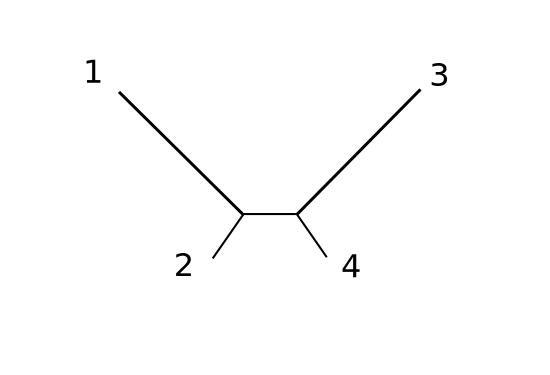
\includegraphics[width=.45\textwidth]{unrooted_four_taxa}
    \caption{Four taxon tree}
\label{fig:four-taxa-tree}
\end{figure}

Consider the fixed, binary four-tip tree $\tau$ in Fig.~\ref{fig:four-taxa-tree}.
The set of all possible character assignments can be described as
\begin{align*}
\mathcal{P}(\{1,2,3,4\}) &= \{\emptyset, \{1,2,3,4\}, \{1\}, \{2,3,4\}, \{2\}, \{1,3,4\}, \{3\}, \{1,2,4\}, \\
                         &\qquad \{1,2\}, \{3,4\}, \{1,3\}, \{2,4\}, \{2,3\}, \{1,4\}, \{1,2,3\}, \{1,4\}\}.
\end{align*}
where each set indicates the tips at which a character is assigned the character $1$.
For example, $\emptyset$ is the labeling $0000$ and $\{1,3,4\}$ is the labeling $1011$.
Symmetry allows us to group adjacent pairs in $\mathcal{P}(\{1,2,3,4\})$ into equiprobable splits, letting $\siteSplitSet=\{1,2,3\}$.
The unique site splits, collapsing complements, are
$$
\mathcal{P}(\siteSplitSet) = \{\emptyset, \{1\}, \{2\}, \{3\}, \{1,2\}, \{1,3\}, \{2,3\}, \{1,2,3\}\}.
$$
Had we not identified character complements, we would need to consider the additional splits
$$
\mathcal{P}(\{1,2,3,4\}) \setminus \mathcal{P}(\siteSplitSet) = \{\{1,2,3,4\}, \{2,3,4\}, \{1,3,4\}, \{1,2,4\}, \{3,4\}, \{2,4\}, \{1,4\}, \{4\}\},
$$
but the symmetry of the binary character model allows us to focus just on the elements of $\mathcal{P}(\siteSplitSet)$.
This tree has two internal nodes with $\ancestralSplitSet=\{1,2\}$ and unique ancestral state splits
$$
\mathcal{P}(\ancestralSplitSet) = \{\emptyset, \{1\}, \{2\}, \{1,2\}\}.
$$
We cannot similarly identify complements in this case since, for $\siteSplit\in\mathcal{P}(\siteSplitSet)$,
$$
P(\ancestralSplitRV=\emptyset \mid \siteSplitRV=\siteSplit, \tau, t)\neq P(\ancestralSplitRV=\{1,2\} \mid \siteSplitRV=\siteSplit, \tau, t)
$$
in general.

For each site split $\siteSplit\in\mathcal{P}(\siteSplitSet)$, we maximize the likelihood over all $\ancestralSplit\in\mathcal{P}(\ancestralSplitSet)$.
A maximum will occur at one of possibly several ancestral splits in $\mathcal{P}(\ancestralSplitSet)$; for the $j$th site split, define $\ancestralSplitPartition_j(\tau, t)\subset\mathcal{P}(\ancestralSplitSet)$ as the set of most likely ancestral splits for that particular site split, topology and set of branch lengths.
As a simple example, say all branch lengths correspond to a probability $p$ ($< 1/2$) of changing character along that branch.
%EM Would it be worth enumerating the site splits ahead of time? It seems a little funky to be calling them j each time.
The probabilities of observing ancestral splits for $\siteSplit_j=\emptyset$ are
$$
P(\ancestralSplitRV=\emptyset \mid \siteSplitRV=\emptyset, \tau, t) =
(1-p)^5,
$$
$$
P(\ancestralSplitRV=\{1\} \mid \siteSplitRV=\emptyset, \tau, t) =
P(\ancestralSplitRV=\{2\} \mid \siteSplitRV=\emptyset, \tau, t) =
p^3(1-p)^2,
$$
$$
P(\ancestralSplitRV=\{1,2\} \mid \siteSplitRV=\emptyset, \tau, t) =
p^4(1-p).
$$
Thus the set of most likely ancestral states contains a single element in this case, here $\ancestralSplitPartition_j(\tau, p)=\{\emptyset\}$.
Then, taking $\xi_j\in\ancestralSplitPartition_j(\tau, p)$ we have
$$
P(\ancestralSplitRV=\xi_j \mid \siteSplitRV=\emptyset, \tau, t) =
(1-p)^5.
$$
For $\siteSplit_j=\{1,3\}$ we have
$$
P(\ancestralSplitRV=\emptyset \mid \siteSplitRV=\{1,3\}, \tau, t) =
P(\ancestralSplitRV=\{1,2\} \mid \siteSplitRV=\{1,3\}, \tau, t) =
p^2(1-p)^3,
$$
$$
P(\ancestralSplitRV=\{1\} \mid \siteSplitRV=\{1,3\}, \tau, t) =
P(\ancestralSplitRV=\{2\} \mid \siteSplitRV=\{1,3\}, \tau, t) =
p^3(1-p)^2.
$$
In this case, the set of most likely ancestral states is $\ancestralSplitPartition_j(\tau, p)=\{\emptyset,\{1,2\}\}$, and, for $\xi_j\in\ancestralSplitPartition_j(\tau, p)$,
$$
P(\ancestralSplitRV=\xi_j \mid \siteSplitRV=\{1,3\}, \tau, t) =
p^2(1-p)^3.
$$

\subsection{Showing inconsistency}

We are interested in the properties of the objective function being maximized in \eqref{eq:site_pattern_likelihood} as data becomes plentiful.
%EM As described IRL, a little strange to be redefining (9) with an extra variable. After reading the below, I think it makes most sense to just refer to (9) indirectly but make this a stand-alone definition.
Define \eqref{eq:site_pattern_likelihood} as
$$
L_\nCols''(\fullAlignment;\fullAncestralSplitPartitions(\tau, t),\tau,t) = \prod_{j=1}^{\nSiteSplits} \ \left[P(\siteSplitRV=\siteSplit_j \mid \tau, t) \cdot P(\ancestralSplitRV=\xi_j \mid \siteSplitRV=\siteSplit_j, \tau, t)\right] ^{\nCols_j(\fullAlignment)}.
$$
Assume our $\nCols$ observations were generated from a model with parameters $(\tau^*, t^*)$.
We have
\begin{align}
    \frac{1}{\nCols} \log L_\nCols''(\fullAlignment;\fullAncestralSplitPartitions(\tau,t),\tau,t)
        &= \sum_{j=1}^\nSiteSplits \frac{\nCols_j(\fullAlignment)}{\nCols}\cdot  \log P(\siteSplitRV=\siteSplit_j, \ancestralSplitRV=\xi_j \mid \tau, t) \\
        &= \sum_{j=1}^\nSiteSplits \frac{\nCols_j(\fullAlignment)}{\nCols}\cdot [\log P(\siteSplitRV=\siteSplit_j \mid \tau, t) +
            \log P(\ancestralSplitRV=\xi_j \mid \siteSplitRV=\siteSplit_j , \tau, t)]
\end{align}
so that, in the limit of infinite data,
\begin{equation}
%EM did you mean to drop the eta from the first term of this equation?
\frac{1}{\nCols} \log L_\nCols''(\fullAlignment;,\tau,t) \rightarrow \sum_{j=1}^\nSiteSplits P(\siteSplitRV=\siteSplit_j \mid \tau^*, t^*) \cdot [\log P(\siteSplitRV=\siteSplit_j \mid \tau, t) + \log P(\ancestralSplitRV=\xi_j \mid \siteSplitRV=\siteSplit_j , \tau, t)]. \label{eq:site_pattern_profile_likelihood_mean}
\end{equation}
Define the the divergence quantity
$$
\shannonDivergence_{\tau^*,t^*}(\tau,t) = \sum_{j=1}^\nSiteSplits P(\siteSplitRV=\siteSplit_j \mid \tau^*, t^*)\cdot\log P(\siteSplitRV=\siteSplit_j \mid \tau, t),
$$
and the partial log likelihood
$$
%EM IMHO \ell^p is so standard that it's confusing to see it in another setting. Perhaps \tilde{\ell}?
\ell^p_{\tau^*,t^*}(\fullAncestralSplitPartitions(\tau,t),\tau,t) = \sum_{j=1}^\nSiteSplits P(\siteSplitRV=\siteSplit_j \mid \tau^*, t^*)\cdot\log P(\ancestralSplitRV=\xi_j \mid \siteSplit_j, \tau, t)
$$
so that \eqref{eq:site_pattern_profile_likelihood_mean} becomes
\begin{equation}
    \label{eq:log_likelihood_simplified}
    \ell_{\tau^*,t^*}(\fullAncestralSplitPartitions(\tau,t),\tau,t) = \shannonDivergence_{\tau^*,t^*}(\tau,t) + \ell^p_{\tau^*,t^*}(\fullAncestralSplitPartitions(\tau,t),\tau,t).
\end{equation}
Recall $(\tau, t)$ are estimands and $(\tau^*, t^*)$ are fixed, generating parameters.
For data generated from $(\tau^*, t^*)$, if
\begin{equation}
\label{eq:inconsistency_inequality}
\ell_{\tau^*,t^*}(\hat{\fullAncestralSplitPartitions}(\tau',t_1),\tau',\hat{t}_1) > \ell_{\tau^*,t^*}(\hat{\fullAncestralSplitPartitions}(\tau^*,t_2),\tau^*,\hat{t}_2)
\end{equation}
for $\tau'\neq\tau^*$ with $\{\hat{t}_1,\hat{\fullAncestralSplitPartitions}(\tau',t_1)\}$ and $\{\hat{t}_2,\hat{\fullAncestralSplitPartitions}(\tau^*,t_2)\}$ estimated by maximizing \eqref{eq:profile_likelihood}, we have an inconsistency.

\section{Inconsistency of joint maximum likelihood}

\subsection{Bounding the likelihoods}

Our approach will be to seek bounds for the terms inside the maximization in \eqref{eq:log_likelihood_simplified} as
\begin{equation}
\label{eq:partial-likelihood}
\ell_{\tau^*,t^*}(\fullAncestralSplitPartitions(\tau,t),\tau,t) = \shannonDivergence_{\tau^*,t^*}(\tau,t) + \ell^p_{\tau^*,t^*}(\fullAncestralSplitPartitions(\tau,t),\tau,t).
\end{equation}
We obtain an upper bound for the joint maximum of \eqref{eq:partial-likelihood}
$$
\max_{t,\fullAncestralSplitPartitions(\tau,t)} \ \ell_{\tau^*,t^*}(\fullAncestralSplitPartitions(\tau,t),\tau,t) \le
    \shannonDivergence_{\tau^*,t^*}(\tau^*,t^*)
+ \ell^p_{\tau^*,t^*}(\hat{\fullAncestralSplitPartitions}(\tau,t),\tau,\hat{t})
$$
using Gibbs's inequality
$$
\shannonDivergence_{\tau^*,t^*}(\tau,t) \le \shannonDivergence_{\tau^*,t^*}(\tau^*,t^*)
$$
and
$$
\{\hat{t},\hat{\fullAncestralSplitPartitions}(\tau,t)\} = \arg\max_{t,\fullAncestralSplitPartitions(\tau,t)} \ \ell^p_{\tau^*,t^*}(\fullAncestralSplitPartitions(\tau,t),\tau,t).
$$
Similarly, we have a lower bound as
$$
\max_{t,\fullAncestralSplitPartitions(\tau,t)} \ \ell_{\tau^*,t^*}(\fullAncestralSplitPartitions(\tau,t),\tau,t) \ge
    \shannonDivergence_{\tau^*,t^*}(\tau,\hat{t})
+ \ell^p_{\tau^*,t^*}(\hat{\fullAncestralSplitPartitions}(\tau,t),\tau,\hat{t}).
$$

% vvvv Remove these? I think they're obvious now, but maybe they can be made more explicit above?
\textbf{Argument for lower bound}: This makes intuitive sense, though may be difficult to show in general.
Can we not just say $\max_u f(u) + g(u)$ is greater than $f(u') + g(u')$ for any $u'$ that doesn't maximize $f(u) + g(u)$ just by definition?
There could be multiple maxima, but that's why we have greater than or equal to.
I think the only thing we'd need to show is that a maximum exists, but since $\{x,y,w\}$ are supported on a closed set this is certainly true.
I must be missing something.

\textbf{Argument for upper bound}: I think this is true mostly because $\max_u f(u) + g(u)$ should be less than $\max_u f(u) + \max_u g(u)$ by some triangle inequality argument.
If we were to actually maximize the full likelihood, we should get something smaller than maximizing some form of it that we consider by looking at the parts separately.
For a fixed $\{x^*, y^*\}$ we can calculate this upper bound directly---can we obtain it as a useful-looking function of these parameters in the general case?

\subsection{Parameter setting}

\begin{figure}
\centering
\begin{subfigure}{.45\linewidth}
\centering
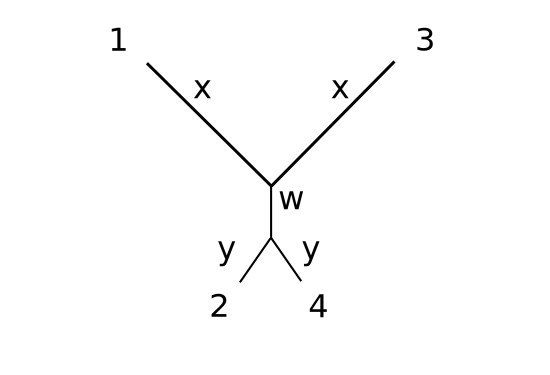
\includegraphics[width=.95\textwidth]{farris_blank}
\caption[short]{Farris topology $\tau_1$}
\end{subfigure}
\begin{subfigure}{.45\linewidth}
\centering
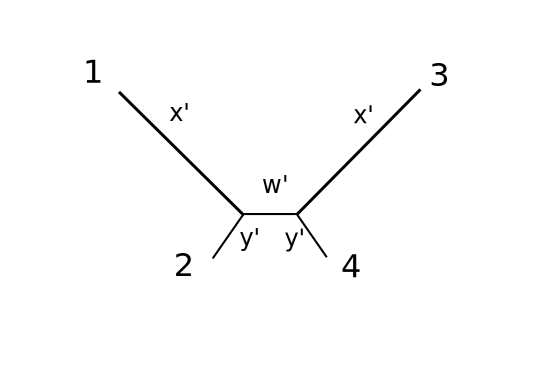
\includegraphics[width=.95\textwidth]{felsenstein_blank}
\caption[short]{Felsenstein topology $\tau_2$}
\end{subfigure}
\caption{Two simple topologies}
\label{fig:farris-fels-top}
\end{figure}

Define the Farris topology $\tau_1$ and the Felsenstein topology $\tau_2$ as in Figure~\ref{fig:farris-fels-top}.
Call $t=\{x,y,w\}$ and $t^*=\{x,y,y\}$, i.e., $t^*$ is the case where the bottom three branches all share the same parameter, the classical construction of this topology.
The branch length parameters are such that the probability of a change in character along the top two branches is $p_x=1-2x$, with corresponding equalities for the other two branches.
Here, $\{p_x,p_y,p_w\}\in[0,1/2]^3$ and $\{x,y,w\}\in[0,1]^3$.

\textbf{Justification for estimand:} It might be worth arguing why this form of the estimand $t$ is necessary.
I think the idea is that for either of these topologies, any maximum obtained will occur where the top two and bottom two branches are equal, though not necessarily the middle branch.
This would be good to show explicitly.

Table~\ref{tab:sitepatprob} contains calculations of site pattern frequencies under these two topologies, calculated using the Hadamard transform approach outlined in 8.6 of Semple and Steel \cite{Semple2003-em}.
Table~\ref{tab:likelihoods} contains calculations of likelihood values for fixed site patterns and topologies, with the maximum values over ancestral state patterns noted.

\begin{table}
\centering
\begin{tabular}{|l|l|l|}
\multicolumn{3}{c}{Classical}\\
    \hline
$\siteSplit_j$   &$P(\siteSplitRV=\siteSplit_j \mid \tau_1,t^*)$&$P(\siteSplitRV=\siteSplit_j \mid \tau_2,t^*)$\\
    \hline
    $\emptyset$    &$1+x^2+y^2+4xy^2+x^2y^2$&$1+2xy+2xy^2+x^2y+y^3+x^2y^2$\\
    $\{1\}$        &$1-x^2+y^2-x^2y^2$&$1-x^2y+y^3-x^2y^2$\\
    $\{2\}$        &$1+x^2-y^2-x^2y^2$&$1+x^2y-y^3-x^2y^2$\\
    $\{3\}$        &$1-x^2+y^2-x^2y^2$&$1-x^2y+y^3-x^2y^2$\\
    $\{1,2\}$      &$1-x^2-y^2+x^2y^2$&$1+2xy-2xy^2-x^2y-y^3+x^2y^2$\\
    $\{1,3\}$      &$1+x^2+y^2-4xy^2+x^2y^2$&$1-2xy-2xy^2+x^2y+y^3+x^2y^2$\\
    $\{2,3\}$      &$1-x^2-y^2+x^2y^2$&$1-2xy+2xy^2-x^2y-y^3+x^2y^2$\\
    $\{1,2,3\}$    &$1+x^2-y^2-x^2y^2$&$1+x^2y-y^3-x^2y^2$\\
    \hline
\multicolumn{3}{c}{Modified}\\
    \hline
$\siteSplit_j$   &$P(\siteSplitRV=\siteSplit_j \mid \tau_1,t)$&$P(\siteSplitRV=\siteSplit_j \mid \tau_2,t)$\\
    \hline
    $\emptyset$     &$1+x^2+y^2+4xyw+x^2y^2$&$1+2xy+2xyw+x^2w+y^2w+x^2y^2$\\
    $\{1\}$        &$1-x^2+y^2-x^2y^2$&$1-x^2w+y^2w-x^2y^2$\\
    $\{2\}$        &$1+x^2-y^2-x^2y^2$&$1+x^2w-y^2w-x^2y^2$\\
    $\{3\}$        &$1-x^2+y^2-x^2y^2$&$1-x^2w+y^2w-x^2y^2$\\
    $\{1,2\}$      &$1-x^2-y^2+x^2y^2$&$1+2xy-2xyw-x^2w-y^2w+x^2y^2$\\
    $\{1,3\}$      &$1+x^2+y^2-4xyw+x^2y^2$&$1-2xy-2xyw+x^2w+y^2w+x^2y^2$\\
    $\{2,3\}$      &$1-x^2-y^2+x^2y^2$&$1-2xy+2xyw-x^2w-y^2w+x^2y^2$\\
    $\{1,2,3\}$    &$1+x^2-y^2-x^2y^2$&$1+x^2w-y^2w-x^2y^2$\\
    \hline
\end{tabular}
\caption{Site pattern probabilities.
All values are multiplied by $1/8$.}
\label{tab:sitepatprob}
\end{table}

\begin{table}
\centering
\begin{tabular}{|l|ll|}
    \multicolumn{3}{c}{$\tau=\tau_1$}\\
    \hline
    $\siteSplit_j$    & $\ancestralSplitPartition_j(\tau, t)$ & $P(\ancestralSplitRV=\xi_j \mid \siteSplitRV=\siteSplit_j,\tau,t)$\\
    \hline
    $\emptyset$&
    $\emptyset$&
    $(1+x)^2   (1+w)(1+y)^2$\\
     $\{1\}$    &
    $\emptyset$&
    $(1+x)(1-x)(1+w)(1+y)^2$\\
     $\{2\}$    &
    $\emptyset$&
    $(1+x)^2   (1+w)(1+y)(1-y)$\\
     $\{3\}$    &
    $\emptyset$&
    $(1+x)(1-x)(1+w)(1+y)^2$\\
    $\{1,2\}$  &
    $\{\emptyset,\{1,2,3\}\}$&
    $(1+x)(1-x)(1+w)(1+y)(1-y)$\\
    $\{1,3\}$  &
    $\left\{\begin{array}{l}
                    \emptyset\\
                    \{2\}\\
                    \{1,2\}
                \end{array}\right.$&
    $\begin{array}{l}
                    (1+x)^2   (1+w)(1-y)^2\\
                    (1+x)^2   (1-w)(1+y)^2\\
                    (1-x)^2   (1+w)(1+y)^2
                \end{array}$\\
    $\{2,3\}$  &
                $\{\emptyset,\{1,2,3\}\}$&
                $(1+x)(1-x)(1+w)(1+y)(1-y)$\\
    $\{1,2,3\}$&
                $\emptyset$&
                $(1+x)^2   (1+w)(1+y)(1-y)$\\
    \hline
    \multicolumn{3}{c}{$\tau=\tau_2$}\\
    \hline
    $\siteSplit_j$    & $\ancestralSplitPartition_j(\tau, t)$ & $P(\ancestralSplitRV=\xi_j \mid \siteSplitRV=\siteSplit_j,\tau,t)$\\
    \hline
    $\emptyset$       &$\emptyset$&$(1+x)^2   (1+w)(1+y)^2$\\
    $\{1\}$          &
    $\left\{\begin{array}{l}
                    \emptyset\\
                    \{1\}
                \end{array}\right.$&
    $\begin{array}{l}
                        (1+x)(1-x)(1+w)(1+y)^2\\
                        (1+x)^2   (1-w)(1+y)(1-y)
                    \end{array}$\\
      $\{2\}$          &
    $\left\{\begin{array}{l}
                    \emptyset\\
                    \{1\}
                \end{array}\right.$&
    $\begin{array}{l}
                    (1+x)^2   (1+w)(1+y)(1-y)\\
                    (1+x)(1-x)(1-w)(1+y)^2
                    \end{array}$\\
      $\{3\}$          &
    $\left\{\begin{array}{l}
                    \emptyset\\
                    \{2\}
                \end{array}\right.$&
    $\begin{array}{l}
                    (1+x)(1-x)(1+w)(1+y)^2\\
                    (1+x)^2   (1-w)(1+y)(1-y)
                    \end{array}$\\
     $\{1,2\}$         &
    $\left\{\begin{array}{l}
                    \{\emptyset,\{1,2\}\}\\
                    \{2\}
                \end{array}\right.$&
    $\begin{array}{l}
                    (1+x)(1-x)(1+w)(1+y)(1-y)\\
                    (1+x)^2   (1-w)(1+y)^2
                    \end{array}$\\
     $\{1,3\}$         &
    $\left\{\begin{array}{l}
                    \emptyset\\
                    \{\{1\},\{2\}\}\\
                    \{1,2\}
                \end{array}\right.$&
    $\begin{array}{l}
                    (1+x)^2   (1+w)(1-y)^2\\
                    (1+x)(1-x)(1-w)(1+y)(1-y)\\
                    (1-x)^2   (1+w)(1+y)^2
                    \end{array}$\\
      $\{2,3\}$        &
    $\left\{\begin{array}{l}
                    \{\emptyset,\{1,2\}\}\\
                    \{1\}\\
                    \{2\}
                \end{array}\right.$&
    $\begin{array}{l}
                    (1+x)(1-x)(1+w)(1+y)(1-y)\\
                    (1-x)^2   (1-w)(1+y)^2\\
                    (1+x)^2   (1-w)(1-y)^2
                    \end{array}$\\
     $\{1,2,3\}$       &
    $\left\{\begin{array}{l}
                    \emptyset\\
                    \{2\}
                \end{array}\right.$&
    $\begin{array}{l}
                    (1+x)^2   (1+w)(1+y)(1-y)\\
                    (1+x)(1-x)(1-w)(1+y)^2
                    \end{array}$\\
    \hline
\end{tabular}
\caption{Likelihood calculations for all site patterns and ancestral state partitions.
All values multiplied by $1/32$.
Likelihoods with multiple entries will have maxima determined by unknown branch length parameters.}
\label{tab:likelihoods}
\end{table}

\subsubsection{Upper bound for Farris partial likelihood}

Assume $\tau^*=\tau_1$ and $t^*=\{x,y,y\}$.
For compactness, define, e.g., $p_0 = P(\siteSplitRV=\emptyset \mid \tau=\tau_1,t=\{x,y,y\})$, keeping in mind it is a function of parameters $x,y$.
The full Farris log likelihood can take one of three values---assume for now the we are only interested in the ancestral state split $\{2\}$ for the site split $\{1,3\}$.
We then write the log likelihood as
\begin{align*}
    \ell_{\tau_1,\{x,y,y\}}(\fullAncestralSplitPartitions(\tau_1,\{x',y',w'\}),\tau_1,\{x',y',w'\})
    &=        p_{0}  \cdot\log(1+x'^2+y'^2+4x'y'w'+x'^2y'^2) \\
    &\qquad + p_{1}  \cdot\log(1-x'^2+y'^2-x'^2y'^2) \\
    &\qquad + p_{2}  \cdot\log(1+x'^2-y'^2-x'^2y'^2) \\
    &\qquad + p_{3}  \cdot\log(1-x'^2+y'^2-x'^2y'^2) \\
    &\qquad + p_{12} \cdot\log(1-x'^2-y'^2+x'^2y'^2) \\
    &\qquad + p_{13} \cdot\log(1+x'^2+y'^2-4x'y'w'+x'^2y'^2) \\
    &\qquad + p_{23} \cdot\log(1-x'^2-y'^2+x'^2y'^2) \\
    &\qquad + p_{123}\cdot\log(1+x'^2-y'^2-x'^2y'^2) \\
    &\qquad + p_{0}  \cdot\log((1+x')^2   (1+w')(1+y')^2) \\
    &\qquad + p_{1}  \cdot\log((1+x')(1-x')(1+w')(1+y')^2) \\
    &\qquad + p_{2}  \cdot\log((1+x')^2   (1+w')(1+y')(1-y')) \\
    &\qquad + p_{3}  \cdot\log((1+x')(1-x')(1+w')(1+y')^2) \\
    &\qquad + p_{12} \cdot\log((1+x')(1-x')(1+w')(1+y')(1-y')) \\
    &\qquad + p_{13} \cdot\log((1+x')^2   (1-w')(1+y')^2) \\
    &\qquad + p_{23} \cdot\log((1+x')(1-x')(1+w')(1+y')(1-y')) \\
    &\qquad + p_{123}\cdot\log((1+x')^2   (1+w')(1+y')(1-y')).
\end{align*}
Seeking an upper bound, we make use of the fact that, for $x',y'\in[0,1]$,
$$
(1-x'^2+y'^2-x'^2y'^2) = (1-x'^2)(1+y'^2) = (1+x')(1-x')(1+y'^2) \le (1+x')(1-x')(1+y),
$$
with similar substitutions for $(1+x'^2-y'^2-x'^2y'^2)$ and $(1-x'^2-y'^2+x'^2y'^2)$.
Doing so results in
\begin{align*}
    \ell_{\tau_1,\{x,y,y\}}(\fullAncestralSplitPartitions(\tau_1,\{x',y',w'\}),\tau_1,\{x',y',w'\})
    &\le      p_{0}  \cdot\log(1+x'^2+y'^2+4x'y'w'+x'^2y'^2) \\
    &\qquad + p_{13} \cdot\log(1+x'^2+y'^2-4x'y'w'+x'^2y'^2) \\
    &\qquad + p_{1}  \cdot\log((1+x')(1-x')(1+y')) \\
    &\qquad + p_{2}  \cdot\log((1+x')(1+y')(1-y')) \\
    &\qquad + p_{3}  \cdot\log((1+x')(1-x')(1+y')) \\
    &\qquad + p_{12} \cdot\log((1+x')(1-x')(1+y')(1-y')) \\
    &\qquad + p_{23} \cdot\log((1+x')(1-x')(1+y')(1-y')) \\
    &\qquad + p_{123}\cdot\log((1+x')(1+y')(1-y')) \\
    &\qquad + p_{0}  \cdot\log((1+x')^2   (1+w')(1+y')^2) \\
    &\qquad + p_{1}  \cdot\log((1+x')(1-x')(1+w')(1+y')^2) \\
    &\qquad + p_{2}  \cdot\log((1+x')^2   (1+w')(1+y')(1-y')) \\
    &\qquad + p_{3}  \cdot\log((1+x')(1-x')(1+w')(1+y')^2) \\
    &\qquad + p_{12} \cdot\log((1+x')(1-x')(1+w')(1+y')(1-y')) \\
    &\qquad + p_{13} \cdot\log((1+x')^2   (1-w')(1+y')^2) \\
    &\qquad + p_{23} \cdot\log((1+x')(1-x')(1+w')(1+y')(1-y')) \\
    &\qquad + p_{123}\cdot\log((1+x')^2   (1+w')(1+y')(1-y')).
\end{align*}
Grouping together like terms,
\begin{align*}
    \ell_{\tau_1,\{x,y,y\}}(\fullAncestralSplitPartitions(\tau_1,\{x',y',w'\}),\tau_1,\{x',y',w'\})
    &\le      p_{0}  \cdot\log(1+x'^2+y'^2+4x'y'w'+x'^2y'^2) \\
    &\qquad + p_{13} \cdot\log(1+x'^2+y'^2-4x'y'w'+x'^2y'^2) \\
    &\qquad + (1-p_{0}-p_{13})\cdot\log(1+x') \\
    &\qquad + (p_{1}+p_{3}+p_{12}+p_{23})\cdot\log(1-x') \\
    &\qquad + (1-p_{0}-p_{13})\cdot\log(1+y') \\
    &\qquad + (p_{2}+p_{12}+p_{23}+p_{123})\cdot\log(1-y') \\
    &\qquad + (2-p_{1}-p_{3}-p_{12}-p_{23})\cdot\log(1+x') \\
    &\qquad + (p_{1}+p_{3}+p_{12}+p_{23})\cdot\log(1-x') \\
    &\qquad + (2-p_{2}-p_{12}-p_{23}-p_{123})\cdot\log(1+y') \\
    &\qquad + (p_{2}+p_{12}+p_{23}+p_{123})\cdot\log(1-y') \\
    &\qquad + (1-p_{13})\cdot\log(1+w') \\
    &\qquad + p_{13}\cdot\log(1-w'),
\end{align*}
which equals
\begin{align*}
    \ell_{\tau_1,\{x,y,y\}}(\fullAncestralSplitPartitions(\tau_1,\{x',y',w'\}),\tau_1,\{x',y',w'\})
    &\le      p_{0}  \cdot\log(1+x'^2+y'^2+4x'y'w'+x'^2y'^2) \\
    &\qquad + p_{13} \cdot\log(1+x'^2+y'^2-4x'y'w'+x'^2y'^2) \\
    &\qquad + (3-p_{0}-p_{13}-p_{1}-p_{3}-p_{12}-p_{23})\cdot\log(1+x') \\
    &\qquad + 2(p_{1}+p_{3}+p_{12}+p_{23})\cdot\log(1-x') \\
    &\qquad + (3-p_{0}-p_{13}-p_{2}-p_{12}-p_{23}-p_{123})\cdot\log(1+y') \\
    &\qquad + 2(p_{2}+p_{12}+p_{23}+p_{123})\cdot\log(1-y') \\
    &\qquad + (1-p_{13})\cdot\log(1+w') \\
    &\qquad + p_{13}\cdot\log(1-w').
\end{align*}
To make matters further compact, let
$$
a_{1} = 3-p_{0}-p_{13}-p_{1}-p_{3}-p_{12}-p_{23},
$$
$$
a_{2} = 2(p_{1}+p_{3}+p_{12}+p_{23}),
$$
$$
a_{3} = 3-p_{0}-p_{13}-p_{2}-p_{12}-p_{23}-p_{123},
$$
$$
a_{4} = 2(p_{2}+p_{12}+p_{23}+p_{123}),
$$
where
\begin{align*}
    \ell_{\tau_1,\{x,y,y\}}(\fullAncestralSplitPartitions(\tau_1,\{x',y',w'\}),\tau_1,\{x',y',w'\})
    &\le      p_{0}  \cdot\log(1+x'^2+y'^2+4x'y'w'+x'^2y'^2) \\
    &\qquad + p_{13} \cdot\log(1+x'^2+y'^2-4x'y'w'+x'^2y'^2) \\
    &\qquad + a_{1}\cdot\log(1+x') \\
    &\qquad + a_{2}\cdot\log(1-x') \\
    &\qquad + a_{3}\cdot\log(1+y') \\
    &\qquad + a_{4}\cdot\log(1-y') \\
    &\qquad + (1-p_{13})\cdot\log(1+w') \\
    &\qquad + p_{13}\cdot\log(1-w').
\end{align*}
Applying Gibbs' inequality to the first two summands and maximizing over the remaining terms yields
\begin{align*}
    \ell_{\tau_1,\{x,y,y\}}(\fullAncestralSplitPartitions(\tau_1,\{x',y',w'\}),\tau_1,\{x',y',w'\})
    &\le      p_{0}  \cdot\log(p_{0}) \\
    &\qquad + p_{13} \cdot\log(p_{13}) \\
    &\qquad + a_{1}\cdot\log\frac{2a_{1}}{a_{1}+a_{2}} \\
    &\qquad + a_{2}\cdot\log\frac{2a_{2}}{a_{1}+a_{2}} \\
    &\qquad + a_{3}\cdot\log\frac{2a_{3}}{a_{3}+a_{4}} \\
    &\qquad + a_{4}\cdot\log\frac{2a_{4}}{a_{3}+a_{4}} \\
    &\qquad + (1-p_{13})\cdot\log(2(1-p_{13})) \\
    &\qquad + p_{13}\cdot\log(2p_{13}) \\
    &\qquad := L^{p,1}_{\tau_1,\tau_1}(\mathbf{p}_{xy}).
\end{align*}

The other two possibilties for the likelihood of the ancestral state split $\{2\}$ for the site split $\{1,3\}$ admit similar simplifications.
Call
$$
a_{1}' = a_{1}-2p_{13},
$$
$$
a_{2}' = a_{2}+2p_{13},
$$
$$
a_{3}' = a_{3}-2p_{13},
$$
$$
a_{4}' = a_{4}+2p_{13}.
$$
Then, for these cases,
\begin{align*}
    \ell_{\tau_1,\{x,y,y\}}(\fullAncestralSplitPartitions(\tau_1,\{x',y',w'\}),\tau_1,\{x',y',w'\})
    &\le      p_{0}  \cdot\log(p_{0}) \\
    &\qquad + p_{13} \cdot\log(p_{13}) \\
    &\qquad + a_{1}'\cdot\log\frac{2a_{1}'}{a_{1}'+a_{2}'} \\
    &\qquad + a_{2}'\cdot\log\frac{2a_{2}'}{a_{1}'+a_{2}'} \\
    &\qquad + a_{3}\cdot\log\frac{2a_{3}}{a_{3}+a_{4}} \\
    &\qquad + a_{4}\cdot\log\frac{2a_{4}}{a_{3}+a_{4}} \\
    &\qquad + \log(2) \\
    &\qquad := L^{p,2}_{\tau_1,\tau_1}(\mathbf{p}_{xy});
\end{align*}
\begin{align*}
    \ell_{\tau_1,\{x,y,y\}}(\fullAncestralSplitPartitions(\tau_1,\{x',y',w'\}),\tau_1,\{x',y',w'\})
    &\le      p_{0}  \cdot\log(p_{0}) \\
    &\qquad + p_{13} \cdot\log(p_{13}) \\
    &\qquad + a_{1}\cdot\log\frac{2a_{1}}{a_{1}+a_{2}} \\
    &\qquad + a_{2}\cdot\log\frac{2a_{2}}{a_{1}+a_{2}} \\
    &\qquad + a_{3}'\cdot\log\frac{2a_{3}'}{a_{3}'+a_{4}'} \\
    &\qquad + a_{4}'\cdot\log\frac{2a_{4}'}{a_{3}'+a_{4}'} \\
    &\qquad + \log(2) \\
    &\qquad := L^{p,3}_{\tau_1,\tau_1}(\mathbf{p}_{xy}).
\end{align*}
All bounds are functions only of $x,y$ through the true generating probabilities $\mathbf{p}_{xy}$.

\subsubsection{Lower bound for Felsenstein partial likelihood}

We construct a similar lower bound on the Felsenstein partial likelihood.
Replace all $(1+w)$ terms with $(1-w)$ and focus just on the partial likelihood.
Then if $(1+x)(1-y) > (1-x)(1+y)$,
\begin{align*}
    \ell^p_{\tau_1,\{x,y,y\}}(\fullAncestralSplitPartitions(\tau_2,\{x',y',w'\}),\tau_2,\{x',y',w'\})
    &=      + p_{0}  \cdot\log((1+x')^2   (1+w')(1+y')^2) \\
    &\qquad + p_{1}  \cdot\log((1+x')^2   (1-w')(1+y')(1-y')) \\
    &\qquad + p_{2}  \cdot\log((1+x')^2   (1-w')(1+y')(1-y')) \\
    &\qquad + p_{3}  \cdot\log((1+x')^2   (1-w')(1+y')(1-y')) \\
    &\qquad + p_{12} \cdot\log((1+x')^2   (1-w')(1+y')^2) \\
    &\qquad + p_{123}\cdot\log((1+x')^2   (1-w')(1+y')(1-y'))\\
    &\qquad + p_{13} \cdot\log((1+x')^2   (1-w')(1-y')^2) \\
    &\qquad + p_{23} \cdot\log((1+x')^2   (1-w')(1-y')^2),
\end{align*}
otherwise
\begin{align*}
    \ell^p_{\tau_1,\{x,y,y\}}(\fullAncestralSplitPartitions(\tau_2,\{x',y',w'\}),\tau_2,\{x',y',w'\})
    &=      + p_{0}  \cdot\log((1+x')^2    (1+w')(1+y')^2) \\
    &\qquad + p_{1}  \cdot\log((1+x')(1-x')(1-w')(1+y')^2) \\
    &\qquad + p_{2}  \cdot\log((1+x')(1-x')(1-w')(1+y')^2) \\
    &\qquad + p_{3}  \cdot\log((1+x')(1-x')(1-w')(1+y')^2) \\
    &\qquad + p_{12} \cdot\log((1+x')^2    (1-w')(1+y')^2) \\
    &\qquad + p_{123}\cdot\log((1+x')(1-x')(1-w')(1+y')^2)\\
    &\qquad + p_{13} \cdot\log((1-x')^2    (1-w')(1+y')^2) \\
    &\qquad + p_{23} \cdot\log((1-x')^2    (1-w')(1+y')^2).
\end{align*}
Letting
$$
b_{1} = p_{1}+p_{2}+p_{3}+p_{123}
$$
yields
\begin{align*}
    \ell^p_{\tau_1,\{x,y,y\}}(\fullAncestralSplitPartitions(\tau_2,\{x',y',w'\}),\tau_2,\{x',y',w'\})
    &=      + 2\cdot\log(1+x') \\
    &\qquad + (2-b_{1})  \cdot\log(1+y') \\
    &\qquad + b_{1}      \cdot\log(1-y') \\
    &\qquad + p_{0}\cdot\log(1+w') \\
    &\qquad + (1-p_{0})\cdot\log(1-w')
\end{align*}
for the first lower bound, but, upon maximizing, we obtain the same value for both cases, namely
\begin{align*}
    \ell^p_{\tau_1,\{x,y,y\}}(\fullAncestralSplitPartitions(\tau_2,\{x',y',w'\}),\tau_2,\{x',y',w'\})
    &=      + 2\cdot\log(2) \\
    &\qquad + (2-b_{1})  \cdot\log(2-b_{1}) \\
    &\qquad + b_{1}      \cdot\log(b_{1}) \\
    &\qquad + p_{0}\cdot\log(2p_{0}) \\
    &\qquad + (1-p_{0})\cdot\log(2(1-p_{0}))
\end{align*}
maximized at $\{1,1-b_{1},1-2p_{0}\}$.

...

$$
    L^{p,1}_{\tau_1,\tau_2}(\mathbf{p}_{xy}) := \shannonDivergence_{\tau_1,\{x,y,y\}}(\tau_2,\{1,1-b_{1},1-2p_{0}\}) +
$$

\subsubsection{Region of inconsistency}

We want to find values for $\{x,y\}$ where all of
$$
\shannonDivergence_{\tau_1,\{x,y,y\}}(\tau_2,\{1, 1-b_{1}-2b_{2}, 0\}) + L^{p,1}_{\tau_1,\tau_2}(b_{1},b_{2}) \ge \shannonDivergence_{\tau_1,\{x,y,y\}}(\tau_1,\{y, y, y\}) + L^{p,1}_{\tau_1,\tau_1}(\mathbf{a}_{xy}),
$$
$$
\shannonDivergence_{\tau_1,\{x,y,y\}}(\tau_2,\{1, 1-b_{1}-2b_{2}, 0\}) + L^{p,1}_{\tau_1,\tau_2}(b_{1},b_{2}) \ge \shannonDivergence_{\tau_1,\{x,y,y\}}(\tau_1,\{y, y, y\}) + L^{p,2}_{\tau_1,\tau_1}(\mathbf{a}_{xy})
$$
and
$$
\shannonDivergence_{\tau_1,\{x,y,y\}}(\tau_2,\{1, 1-b_{1}-2b_{2}, 0\}) + L^{p,1}_{\tau_1,\tau_2}(b_{1},b_{2}) \ge \shannonDivergence_{\tau_1,\{x,y,y\}}(\tau_1,\{y, y, y\}) + L^{p,3}_{\tau_1,\tau_1}(\mathbf{a}_{xy})
$$
hold.
Since these are three inequalities in two variables, we can plot them analytically---see Fig.~\ref{fig:inconsistency-farris}.

\begin{figure}
\centering
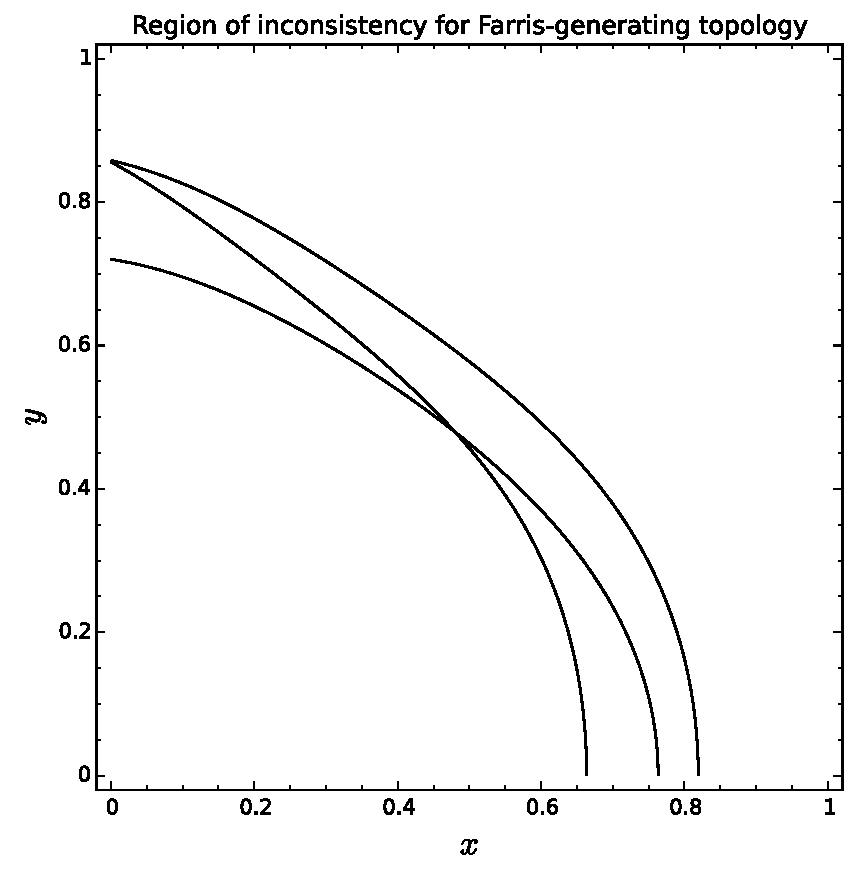
\includegraphics[width=.9\textwidth]{analytic-inconsistency}
\caption{
    Regions of inconsistency.
    Due to the looseness of the upper and lower bounds, the parameters in the top right do not necessarily indicate consistency, though all parameters in the labeled region will result in an inconsistency.
}
\label{fig:inconsistency-farris}
\end{figure}

\paragraph{Examples}

See Table~\ref{tab:examples} for parameters, bounds and true likelihood values obtained via basin hopping.

Set $\{x, y\} = \{0.25, 0.25\}$.
For a Farris zone generating topology, we have
$$
L^{p,1}_{\tau_1,\tau_1}(\mathbf{a}_{xy}) \approx -2.17803560694157,
$$
$$
L^{p,2}_{\tau_1,\tau_1}(\mathbf{a}_{xy}) \approx -2.17803560694157
$$
and
$$
L^{p,3}_{\tau_1,\tau_1}(\mathbf{a}_{xy}) \approx -2.17803560694157.
$$
Computing the upper bound yields
$$
\max_{t,\fullAncestralSplitPartitions(\tau_1,t)} \ \ell_{\tau_1,\{x,y,y\}}(\fullAncestralSplitPartitions(\tau_1,t),\tau_1,t) \le -4.22274479428471
$$
and it remains to show that
$$
\max_{t,\fullAncestralSplitPartitions(\tau_2,t)} \ \ell_{\tau_1,\{x,y,y\}}(\fullAncestralSplitPartitions(\tau_2,t),\tau_2,t) \ge -4.22274479428471.
$$

For the same generating parameters,
$$
d_{xy} = 0.498046875, \ e_{xy} = 0.2431640625,
$$
resulting in
$$
L^{p,1}_{\tau_1,\tau_2}(d_{xy},e_{xy}) \approx -2.07968569223991
$$
and
$$
\shannonDivergence_{\tau_1,\{x,y,y\}}(\tau_2,\{1, 1-d_{xy}-2e_{xy}, 0\}) \approx -2.07748833719921.
$$
The lower bound in this case becomes
$$
\max_{t,\fullAncestralSplitPartitions(\tau_2,t)} \ \ell_{\tau_1,\{x,y,y\}}(\fullAncestralSplitPartitions(\tau_2,t),\tau_2,t) \ge -4.15717402943912
\ge -4.22274479428471 \ge \max_{t,\fullAncestralSplitPartitions(\tau_1,t)} \ \ell_{\tau_1,\{x,y,y\}}(\fullAncestralSplitPartitions(\tau_1,t),\tau_1,t)
$$
where site patterns are generated from the Farris zone topology.
Confirming, run \texttt{python}'s numerical optimization solver for $\{.25, .25\}$.
Since we are computing a constrained maximization, we can find a global maximum using basin hopping, and doing so yields
$$
\max_{t,\fullAncestralSplitPartitions(\tau_1,t)} \ \ell_{\tau_1,\{x,y,y\}}(\fullAncestralSplitPartitions(\tau_1,t),\tau_1,t) \approx -4.5101771294218045
$$
and
$$
\max_{t,\fullAncestralSplitPartitions(\tau_2,t)} \ \ell_{\tau_1,\{x,y,y\}}(\fullAncestralSplitPartitions(\tau_2,t),\tau_2,t) \approx -4.1544859851260281.
$$
It looks like the lower bound is tighter than the upper bound, so we may try focusing there.

\section{Discussion}

Neyman-Scott paradox.

Interesting that here we are simulating on the Farris tree and end up with the Felsenstein tree.
For maximum parsimony it's the opposite \cite{Felsenstein1978-rr}.
Discussion of number of parameters of each.

However, note that \cite{Siddall1998-hq} get things going the same way, although \cite{Swofford2001-hr} show that the problem is that they didn't simulate long enough sequences.

\bibliographystyle{plain}
\bibliography{joint_inf}

\end{document}
